
Initial version of the program attempted to collapse the wave of cells in sequential order, each row will be collapsed from left to right, then the next row. Although the algorithm can return a correct solution, this poses the problem of the resultant image showing diagonal patterns since the constraints of states consistantly start from one direction to another. 

To enable pseudo random ordering without repeatedly check on cells or keep track of all cells in a queue, modulo addition of prime number is used. As suggested on similar discussion on Stack Overflow \cite{modulo_addition}, modulo addition of a prime number larger than dimension of the array can jump the indices without repeating or missing any in a full set of iterations. 

\begin{figure}[!htb]
    \minipage{0.48\textwidth}
    \centering
    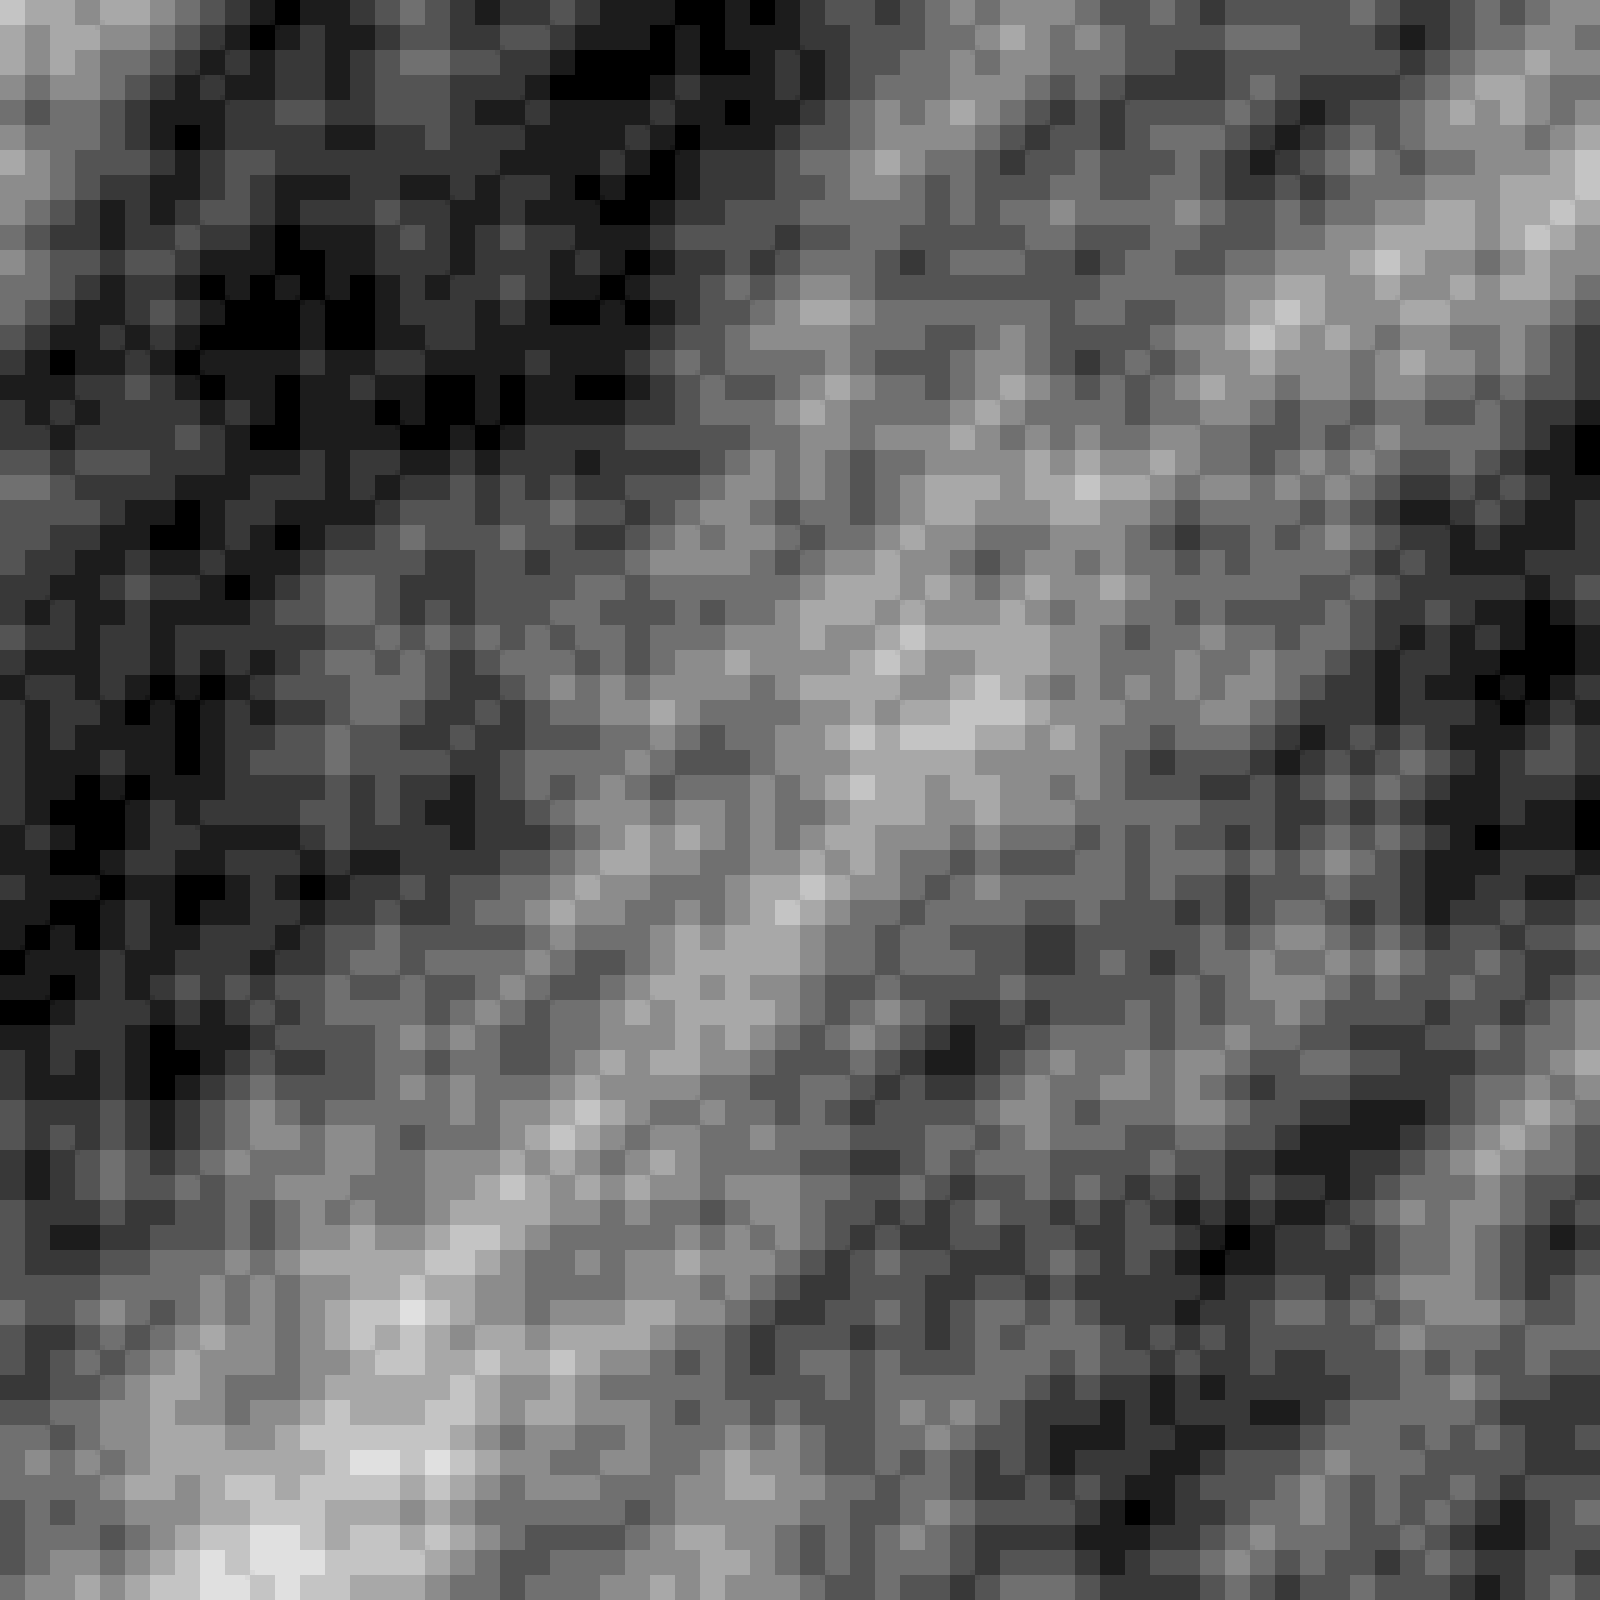
\includegraphics[height=6cm,keepaspectratio]{images/saved_result (scan).png}
    \caption{Collapsed in sequential order}
    \endminipage\hfill
    \minipage{0.48\textwidth}
    \centering
    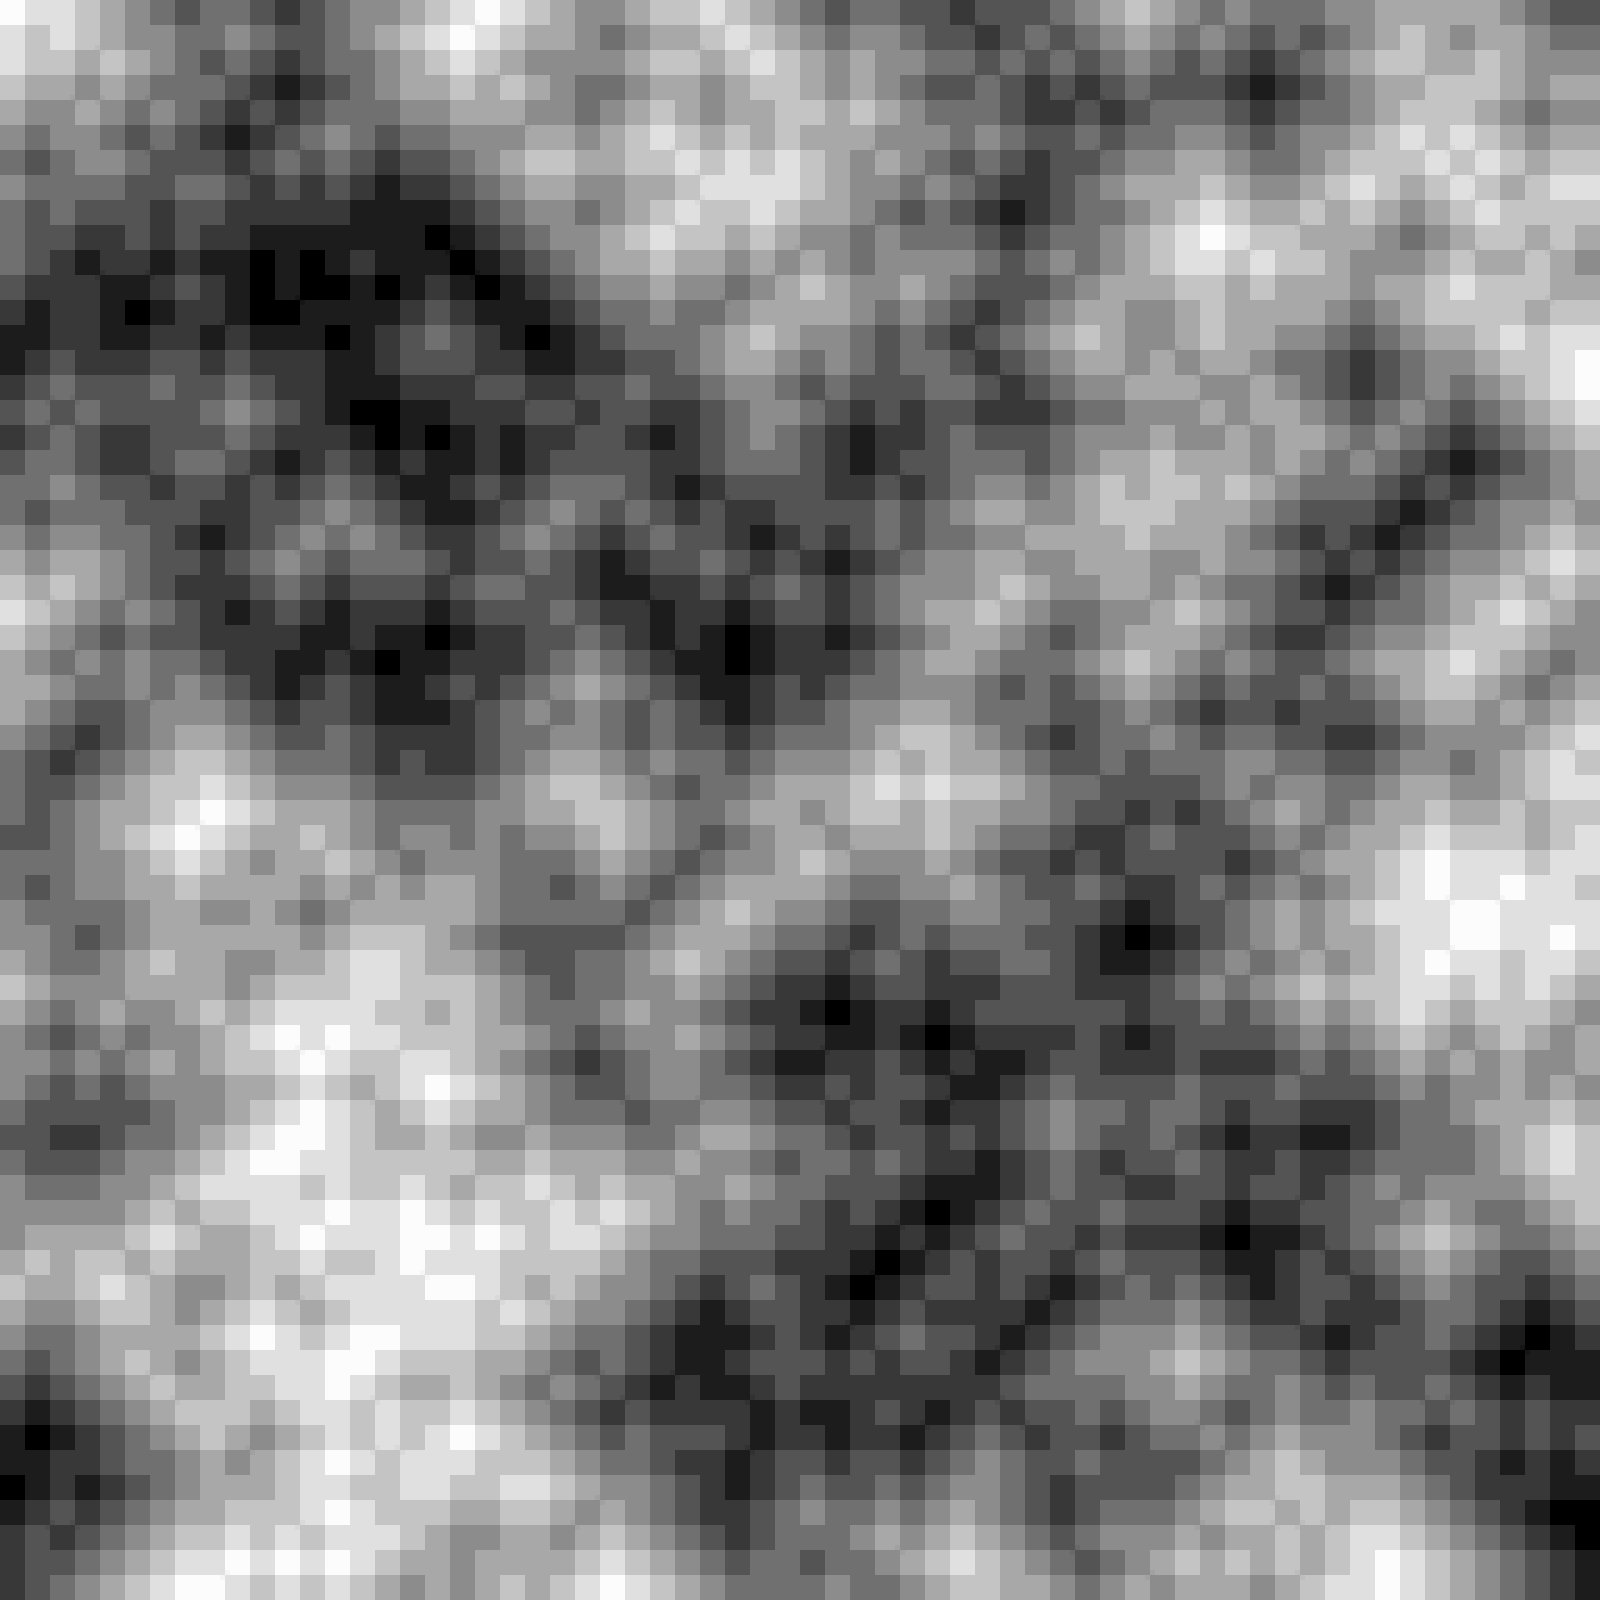
\includegraphics[height=6cm,keepaspectratio]{images/saved_result 64_2.png}
    \caption{Collapsed in modulo addition order}
    \endminipage\hfill
\end{figure}

My algorithm implemented a two-dimensional version of this modulo addition indexing which allows for much more organic results as can be seen in the figures above with minimal computational cost.